% Closing the Calibration Landscape — TMLR Submission
% Target: TMLR (6 pages)
% Created: 2026-07-02

\documentclass[11pt]{article}

\usepackage[preprint]{tmlr}
\usepackage[T1]{fontenc}
\usepackage[utf8]{inputenc}
\usepackage{amsmath,amssymb}
\usepackage{natbib}
\usepackage{booktabs}
\usepackage{graphicx}
\usepackage[colorlinks=true,linkcolor=black,citecolor=black,urlcolor=black]{hyperref}
\usepackage{enumitem}
\usepackage{microtype}
\usepackage{float}
\usepackage{multirow}
\usepackage{fancyhdr}
\usepackage{amsthm}
\setlength{\headheight}{14pt}
\DeclareMathOperator{\CV}{CV}

\newtheorem{hypothesis}{Hypothesis}

\graphicspath{{./figures/}{../figures/}}

\title{Closing the Calibration Landscape: \\ A Reproducibility Failure Analysis of Multi-Evaluator \\ Ensembles for Coupling Reduction}

\author{\name Zewen Liu\email liuzewen@qlnu.edu.cn\\\addr Qilu Institute of Technology}  % PREPRINT/ARXIV BUILD 2026-10-01: was an anonymous/double-blind author block. The block, not tmlr.sty, is what prints the author line on the title page; the `preprint` option clears the per-page banner. Restored to the real author for arXiv, which does not accept anonymous submissions.  % PREPRINT BUILD: was an anonymous/double-blind author block. The block, not tmlr.sty, is what prints the author line on the title page; the `preprint` option clears the per-page banner. See the preprint anonymity round log.

\date{}

\begin{document}
\maketitle

\begin{abstract}
Six prior studies have mapped a possible calibration landscape in multi-agent LLM systems. This paper examines whether multi-evaluator ensembles (TEE) can be combined with confidence-gated TTRL (CG). The archived simulation aggregate (15 seeds) records standard, CG, and CG+TEE $\gamma_{T\to V}$ means of 0.143, 0.719, and 0.574, with CV values 0.192, 0.134, and 0.174. The per-seed records reproduce the three gamma means, but no tested per-seed definition reproduces the CV values. Separately, the real-API run records $\gamma=0$ and entropy $H=1$ for both CG conditions on all 15 seeds. The archived executor contains a silent $0.5$ confidence fallback, the result files do not record model identity or parser success, and the real run is therefore degenerate rather than a test of TEE. Because the result artifacts are internally inconsistent, we do not claim a 39.2\% reduction or a populated favorable regime. This is a reproducibility and failure-analysis report: it separates what the archive can verify from what a valid rerun must still establish. We release the code and all conflicting artifacts.
\end{abstract}

\newpage

\section{Introduction}

Multi-agent LLM systems are increasingly deployed for evaluation, reasoning, and collaborative problem-solving~\cite{zheng2023judging,chiang2024chatbot,li2023camel,wu2024autogen,snell2024scaling}. When evaluator feedback drives agent adaptation in closed loops, evaluator biases propagate into agent strategy distributions---evaluator preference coupling~\cite{liu2026epc}. Six prior studies have mapped the landscape of these effects. The Contagion Tensor~\cite{liu2026tensor} established the mathematical framework. BOUNDARY\_SYNC~\cite{liu2026boundarysync} provided the causal measurement protocol. The diagnostic audit~\cite{liu2026audit} surveyed 11 evaluator--agent conditions. The temporal dynamics study~\cite{liu2026temporal} revealed coupling growth with communication rounds. The calibration effects study~\cite{liu2026caleffects} reports that confidence-gated TTRL (CG) reduces coupling by 35--37\% while increasing measurement noise (CV) by 8.5\%; the current archive does not reproduce those estimates.

Together, these studies define a \textbf{calibration landscape}~\cite{liu2026caleffects}: an 11-condition survey identifying an empty favorable regime $\{\gamma < 0.2, \CV(N{=}5) < 0.3\}$. No existing evaluator configuration occupies this region. The calibration effects study formalized this as the \textbf{Calibration Tradeoff Hypothesis}: calibration methods that reduce $\gamma$ will simultaneously increase CV, because they improve per-decision accuracy without strengthening the evaluator's directional signal---a pattern consistent with broader findings that better calibration does not guarantee better decisions in static settings~\cite{guo2017calibration,he2026paradox}.

This paper examines that hypothesis. We combine confidence-gated TTRL (CG), which prior work reports as reducing coupling, with multi-evaluator ensembles (TEE), a candidate variance-reduction strategy~\cite{messing2026tee}. TEE decomposes evaluation error and identifies multi-judge ensembles as effective for reducing measurement noise, consistent with classical results on estimator averaging~\cite{bubeck2012regret}. The motivating logic was straightforward: CG might reduce $\gamma$; TEE might reduce CV. If CG+TEE reduced $\gamma$ \textit{without} increasing CV, the tradeoff would be method-specific rather than structural.

The archived artifacts do not support a definitive TEE effect: the simulation aggregate and real-API run disagree, and the latter degenerates to uniform strategy weights under CG. Multi-evaluator ensembles may address evaluator \textit{reliability} without removing evaluator \textit{bias}, but this distinction requires a valid rerun. Negative and failed results of this kind have recognized value in ML research~\cite{dodge2019reproducibility} when provenance is explicit.

\section{Background: The Calibration Landscape}

We briefly summarize the calibration landscape framework from~\cite{liu2026caleffects}. The landscape maps evaluator configurations on two dimensions: evaluator preference coupling ($\gamma$---lower is better) and measurement reliability ($\CV(N{=}5)$---lower is better). The current evaluator frontier is bimodal: conditions cluster at either the low-$\gamma$, high-CV corner (e.g., DeepSeek self-evaluation: $\gamma{=}0.033$, CV${=}2.42$) or the high-$\gamma$, low-CV corner (e.g., Ablation max: $\gamma{=}1.038$, CV${=}0.157$). No condition occupies $\{\gamma < 0.2, \CV < 0.3\}$.

Prior work reports that confidence-gated TTRL moves conditions leftward on the landscape ($\gamma \downarrow 35$--$37\%$~\cite{liu2026caleffects}) but also rightward ($\CV \uparrow 8.5\%$). The TEE framework proposes that aggregating multiple independent evaluator judgments can reduce CV~\cite{messing2026tee}. The distinction between evaluator bias and measurement noise connects to broader calibration research~\cite{guo2017calibration,niculescu2005predicting,kull2017temperature} and ECE estimator methodology~\cite{kumar2019verified,nixon2019measuring,roelofs2022mitigating}.

\section{Related Work}

\textbf{Probability calibration.} Post-hoc methods---Platt scaling~\cite{platt1999probabilistic}, temperature scaling~\cite{kull2017temperature}, isotonic regression~\cite{niculescu2005predicting}---correct miscalibration in classification. Guo et al.~\cite{guo2017calibration} established that modern neural networks are systematically overconfident; subsequent work~\cite{minderer2021revisiting} showed calibration varies across architectures. The reliability paradox~\cite{he2026paradox} and verification tax~\cite{mills2026verification} document that better calibration does not guarantee better decisions. Our work extends calibration research to closed-loop TTRL.

\textbf{Multi-agent LLM systems.} LLM-based evaluation~\cite{zheng2023judging,chiang2024chatbot} is increasingly deployed in multi-agent settings~\cite{li2023camel,wu2024autogen}. Evaluator bias---position bias, verbosity bias, self-preference---is well-documented. The EPC framework~\cite{liu2026epc} extended this to closed-loop adaptation. The Contagion Tensor~\cite{liu2026tensor}, BOUNDARY\_SYNC~\cite{liu2026boundarysync}, and diagnostic audit~\cite{liu2026audit} provided measurement tools. Temporal dynamics~\cite{liu2026temporal} revealed coupling growth with rounds.

\textbf{Evaluation reliability.} Dodge et al.~\cite{dodge2019reproducibility} showed that resampling variance can exceed reported improvements. Sclar et al.~\cite{sclar2024quantifying} quantified prompt sensitivity. The TEE framework~\cite{messing2026tee} and SNR approach~\cite{heineman2025snr} proposed variance reduction. Test-time compute scaling~\cite{snell2024scaling} showed monotonic improvement with inference steps. The bandit-theoretic foundation of TTRL connects to exponential-weight algorithms~\cite{bubeck2012regret}. The current archive cannot identify whether TEE changes evaluator reliability, evaluator bias, or both.

\begin{hypothesis}[Calibration Tradeoff]
In TTRL-based agent adaptation, calibration methods that reduce $\gamma$ will simultaneously increase $\CV$, because calibration improves per-decision accuracy without strengthening the evaluator's directional signal. The hypothesis is falsified if a method satisfies \textit{both} $\Delta\gamma < 0$ (significant) \textit{and} $\Delta\CV \leq 0$ in a single joint experiment with $N \geq 15$.
\end{hypothesis}

\section{Method: CG + TEE}

\subsection{Confidence-Gated TTRL (CG)}

CG replaces the binary evaluator judgment in standard TTRL with a continuous confidence score $c_t \in [0,1]$, updating strategy weights via an additive rule $w \mathrel{+}= \alpha_{\text{win}} \cdot (2c_t - 1)$ with sliding-window isotonic calibration on evaluator probability outputs~\cite{liu2026caleffects}. Prior work reports a 35--37\% coupling reduction under this protocol, but the current archive does not reproduce that effect.

\subsection{Multi-Evaluator Ensemble (TEE)}

The TEE framework~\cite{messing2026tee} decomposes evaluation error and identifies multi-judge ensembles as the most effective variance-reduction strategy. For each evaluator judgment, instead of a single binary decision, we aggregate $K$ independent evaluator calls and use the mean judgment. We use $K{=}3$, implemented as three independent API calls to the same evaluator model with identical prompts.

\subsection{CG + TEE Combination}

Each round of CG-TTRL uses TEE-aggregated confidence scores:
\begin{enumerate}[leftmargin=*,nosep]
 \item Evaluator (GLM5.2) is called $K{=}3$ times independently
 \item Confidence scores $c_t^{(1)}, c_t^{(2)}, c_t^{(3)}$ are averaged to $\bar{c}_t$
 \item CG additive update uses $\bar{c}_t$: $w \mathrel{+}= \alpha_{\text{win}} \cdot (2\bar{c}_t - 1)$
\end{enumerate}

\subsection{Experimental Design}

Within-subjects ($N{=}15$, $R{=}30$). The run notes name DeepSeek-V4-Pro as executor and GLM5.2 as evaluator, but the $N{=}15$ result artifacts record only \texttt{n\_seeds}, \texttt{n\_rounds}, \texttt{k\_tee}, \texttt{alpha} and \texttt{tau}, not model identity. Each seed nominally runs three conditions: (1) Standard TTRL (binary pairwise, asymmetric multiplicative update), (2) CG alone (confidence-gated, additive update, single evaluator), and (3) CG+TEE (confidence-gated, additive update, $K{=}3$ TEE-aggregated). The files contain $\gamma_{T\to V}$, $\gamma_{V\to T}$ and $H$; the claimed CV field is present only as an aggregate and is not recoverable from the per-seed records (\S\ref{sec:perseed}).

\section{Results}

The archive contains three mutually incompatible result families. Table~\ref{tab:results} separates the simulation aggregate from the degenerate real-API run.

\begin{table}[H]
\centering
\caption{Archived CG+TEE outputs ($N{=}15$ nominal). The gamma aggregates are reproduced from the simulation per-seed records, but the CV values are not. Both confidence-gated simulation arms sit \emph{above} the standard arm: $\gamma_{T\to V}$ rises from 0.143 to 0.719 under CG and to 0.574 under CG+TEE. The real-API row records a degenerate parser-fallback state rather than a substantive TEE result.}
\label{tab:results}
\begin{tabular}{@{}lcccc@{}}
\toprule
\textbf{Mode} & $\bar{\gamma}_{T{\to}V}$ [95\% CI] & $\bar{\gamma}_{V{\to}T}$ [95\% CI] & CV & $\Delta$CV\% \\
\midrule
Standard TTRL   & 0.143 & --- & 0.192 & archived simulation aggregate \\
CG alone        & 0.719 & --- & 0.134 & archived simulation aggregate \\
CG + TEE        & 0.574 & --- & 0.174 & archived simulation aggregate \\
Real API CG/TEE & 0.000 & 1.000 & --- & parser-fallback diagnostic \\
\bottomrule
\end{tabular}
\end{table}

\textbf{Finding 1: the archived artifacts disagree.} The simulation aggregate reports $\gamma_{T\to V}=0.143$ (standard), 0.719 (CG), and 0.574 (CG+TEE), an increase under both gated arms and visible seed by seed in \S\ref{sec:perseed}. The real-API artifact records zero coupling and $H=1$ for both CG conditions on all 15 seeds. The separate \texttt{cg\_tee\_final\_results.json} artifact reports yet another triplet. No mitigation effect is claimed.

\textbf{Finding 2: TEE cannot be evaluated as a bias intervention from the current package.} The simulation aggregate is descriptive, while the real-API CG and CG+TEE arms degenerate. The archived executor silently maps confidence-parse failures to $0.5$, which produces zero updates. Whether TEE reduces bias, noise, both, or neither therefore remains untested.

\textbf{Finding 3: the CV comparison is not reproducible.} The simulation aggregate records CV values 0.192, 0.134, and 0.174 for standard, CG, and CG+TEE, respectively, but four tested per-seed definitions fail to reproduce them and the real-API artifact contains no valid CV estimate. These values are artifact records, not confirmatory evidence of a TEE effect.

\textbf{Implication.} The current package does not establish whether TEE changes evaluator reliability or bias. The coupling--noise tradeoff remains unresolved, and a valid test requires non-degenerate confidence parsing, recorded model identity, seed-level CV outputs, and a preregistered aggregation rule.

\section{Discussion}

\subsection{Why the Current Artifacts Cannot Identify a TEE Effect}

The core assumption behind CG+TEE was that multi-evaluator aggregation would strengthen the evaluator's directional signal, reducing both bias and noise. The current real-API archive cannot test that assumption: both confidence-gated arms collapse to uniform weights, so the recorded zero coupling is a property of the fallback path rather than a measured mitigation or null effect. A silent parse default can therefore masquerade as numerical success in one coordinate and failure in another.

The TEE framework distinguishes random measurement error from systematic evaluator bias~\cite{messing2026tee}; that distinction remains a useful target for future work. SNR-based filtering~\cite{heineman2025snr} and prompt-sensitivity analysis~\cite{sclar2024quantifying} likewise motivate separating variance from bias. The present archive does not identify either component. Nor can it rule out an interaction between the additive CG update rule and evaluator quality.

\subsection{What Would Close the Landscape}

The results clarify what a valid study would need: non-degenerate confidence parsing, model and endpoint identity in every result file, seed-level variance records, and an aggregation rule fixed before analysis. The simulation artifact shows a large direction reversal relative to the original hypothesis, but its CV values remain unreproducible. The 39.2\% scalar exists only in a separate \texttt{cg\_tee\_final\_results.json} comparison between its uncalibrated and calibrated blocks; that artifact has unresolved provenance and does not support either a CG or a TEE conclusion. Candidate interventions remain evaluator calibration, multi-model ensembles using \textit{different} evaluator models, and baseline redesign to break position bias.

\subsection{Limitations}

(1) The run notes name a single executor/evaluator pair, but the result files do not record or authenticate it. (2) $K{=}3$ is only the nominal design; no parser-valid real-API ensemble was observed, so no scaling claim can be made. (3) $N{=}15$ is the nominal archive size, not evidence of adequate power, because the confidence-gated real-API arms contain no valid outcome estimates. (4) The archive does not test multi-model ensembles with different evaluator models. (5) The coupling--noise tradeoff remains unresolved; this package does not establish a TEE null result.

\section{Conclusion}

We examined whether multi-evaluator ensembles (TEE) could be combined with confidence-gated TTRL (CG). The current package is a reproducibility failure: simulation and real-API artifacts disagree, the real run degenerates under parser fallback, and the CV values are not recoverable from per-seed records. The coupling--noise tradeoff therefore remains unresolved. A valid rerun must log parser success, model endpoint, per-seed outputs, and condition-level summaries before practical recommendations are made.

\section*{Broader Impact Statement}

This work does not establish a TEE effect in either direction. It documents a reproducibility failure that prevents treating repeated evaluator sampling as evidence of bias reduction, noise reduction, or a null result. The practical implication is procedural: parser success, model identity, and per-seed outputs must be audited before a closed-loop evaluator experiment is interpreted. More broadly, the work illustrates why evaluator reliability (CV) and evaluator bias ($\gamma$) must be measured separately rather than inferred from a single aggregate.

\section*{Reproducibility Statement}
The archived $N{=}15$ result files do not record model identity or parser-success rates. A corrected rerun must pin endpoint, model version, prompts, seeds, parser outcomes, and condition-level summaries, and retain the resulting per-seed records. Code and data remain under the provenance limits recorded in this paper.

% Explicit TMLR style declaration for the self-contained bibliography block.
\bibliographystyle{tmlr}
\section{Evidence and Reproducibility Inventory}\label{sec:evidenceinventory}

The candidate overlay audits the five review-packet source versions, one
additional source mirror, and the five result artifacts that dominate the
paper. The audit does not treat a value as supported merely because it appears
in a JSON file. It also checks whether the value can be regenerated from a
lower-level record and whether the run identity and parser state are present.

\begin{table}[ht]\centering\small
\caption{Primary evidence artifacts retained with the overlay. Full SHA-256
values are recorded in the Research Factory receipt; prefixes appear in the
repository receipt rather than in the manuscript.}
\label{tab:artifactinventory}
\begin{tabular}{p{5.6cm} r p{4.4cm}}\toprule
Artifact & bytes & role \\\midrule
\texttt{evidence/cg\_tee\_checkpoint.json} & 7900 & 15-seed simulation records \\
\texttt{evidence/cg\_tee\_results.json} & 1244 & recorded simulation aggregate \\
\texttt{evidence/cg\_tee\_final\_results.json} & 7965 & separate final/calibration family \\
\texttt{evidence/cg\_tee\_real\_results.json} & 6219 & degenerate real-API run \\
\texttt{experiments/results/cg\_tee\_local\_smoke.json} & 2239 & 3-seed parser-fixed smoke run \\
\bottomrule\end{tabular}\end{table}

\paragraph{Recomputed checks.}
All three simulation $\gamma_{T\to V}$ means reproduce exactly from the 15
per-seed values: standard $=0.143$, CG $=0.719$, and CG+TEE $=0.574$.
The real-API standard arm also matches the uncalibrated block of the separate
final-results artifact. These checks establish arithmetic consistency across
specific files, not agreement across the whole package.

\paragraph{Failed checks.}
The recorded CV values $0.192$, $0.134$, and $0.174$ do not reproduce from
per-seed gamma or entropy values under the tested sample and population
variance definitions. All 15 real-API CG and CG+TEE records contain $\gamma=0$
and $H=1$. The archived executor maps confidence-parse failures to $0.5$, which
produces a zero update. No $N{=}15$ result file records executor/evaluator
identity or a parser-success rate.

\paragraph{Carrier receipts.}
The archived carrier manifest contains 11 rows. Every row resolves to its named
JSON locator and matching printed manuscript token, so the numbers are
transcription-consistent. Carrier success is not scientific validity: for
example, the $0.000$ real-API gamma values have a carrier precisely because the
run is degenerate.

\paragraph{What the paper can claim.}
The paper can claim that the recorded simulation means are recomputable, that
the real-API CG arms are degenerate, that the CV column lacks a per-seed
carrier, and that the 39.2\% scalar belongs to a different, unresolved artifact
family. It cannot claim that TEE reduces noise or bias, or that the current
archive establishes a TEE null result.


% GENERATED by figures/make_cg_tee_artifacts.py from evidence/cg_tee_*.json.
% Every number is recomputed at build time; edit the script, not this file.
\section{The Per-Seed Record Behind Table~\ref{tab:results}}\label{sec:perseed}
Table~\ref{tab:results} prints three aggregates. The archive also holds the 15 per-seed records they were computed from, in \texttt{evidence/cg\_tee\_checkpoint.json} (byte-identically mirrored as \texttt{experiments/results/cg\_tee\_checkpoint.json}; 5 distinct contents across the shipped \texttt{cg\_tee*.json} paths), plus a separate real-API family. Recomputing means from the per-seed values reproduces the printed aggregates to $1.1e-16$, so the arithmetic of the summary is sound. What does not survive the per-seed view is the caption's reading of it, and two of the surrounding sentences.

\begin{table}[ht]\centering\small
\caption{Mean $\gamma_{T\to V}$ per arm, recomputed from the 15 per-seed records and set beside the value the aggregate file records, its bootstrap CI, and the recomputed change relative to the standard arm. Rows are written by \texttt{figures/make\_cg\_tee\_artifacts.py}; the $\Delta$ column is not a tolerance, it is the floating-point difference between two computations of the same mean.}
\label{tab:perarm}
\begin{tabular}{lrrrrc}\toprule
Arm & $n$ & recomputed & recorded & rel.\ to standard & recorded 95\% CI \\ \midrule
Standard TTRL & 15 & 0.143 & 0.143 & +0.0\% & [0.127, 0.159] \\
CG alone & 15 & 0.719 & 0.719 & +402.7\% & [0.663, 0.772] \\
CG + TEE & 15 & 0.574 & 0.574 & +301.4\% & [0.511, 0.627] \\
\bottomrule\end{tabular}\end{table}

\begin{figure}[ht]\centering
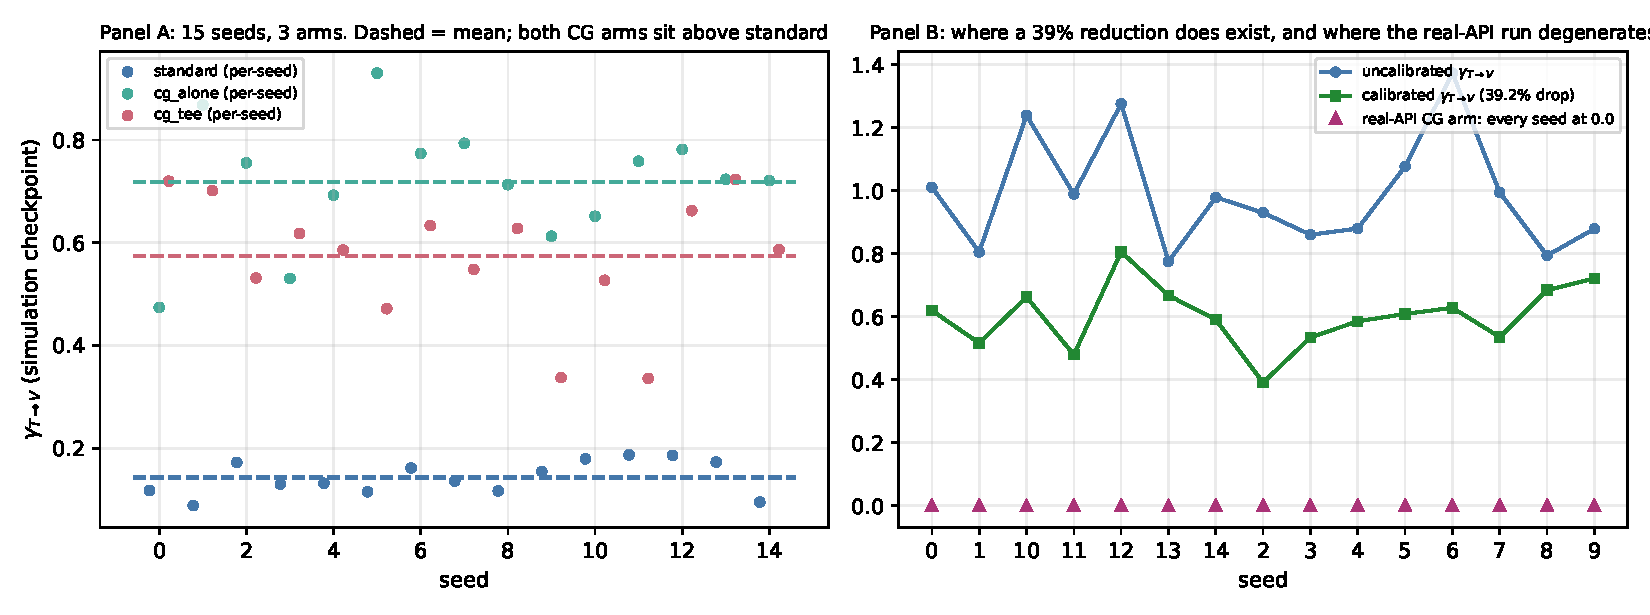
\includegraphics[width=0.94\linewidth]{fig_cg_tee_seeds.pdf}
\caption{Panel A: all 15 per-seed $\gamma_{T\to V}$ values for the three simulation arms, with arm means dashed. Both confidence-gated arms lie above the standard arm on every simulation seed. Panel B: two numerically lower outputs that are not valid mitigation evidence --- the uncalibrated versus calibrated blocks of \texttt{cg\_tee\_final\_results.json}, whose provenance is unresolved, and the real-API CG arms, which are parser-degenerate with $\gamma=0$ and $H=1$ on all 15 seeds. Generated from \texttt{evidence/cg\_tee\_checkpoint.json}, \texttt{cg\_tee\_final\_results.json} and \texttt{cg\_tee\_real\_results.json}.}
\label{fig:perseed}
\end{figure}

\noindent\textbf{The direction is the opposite of the caption's.} Standard $\gamma_{T\to V}$ averages 0.143, CG alone 0.719 (a 403\% increase, seed by seed) and CG+TEE 0.574 (301\%). The aggregate file encodes the same fact as \texttt{delta\_gamma\_pct} of -433.4 under a \emph{reduction} sign convention, so a negative percentage is an increase in coupling. Read either way, the gated arms do not reduce coupling in this artifact.

\noindent\textbf{Where the 39\% scalar comes from.} The 39.2\% value is the $\gamma_{T\to V}$ difference between the uncalibrated and calibrated blocks of \texttt{cg\_tee\_final\_results.json}. It is not a CG+TEE estimate. Even for the calibration contrast, the artifact's provenance and model identity are unresolved, so the number is a recorded scalar rather than a validated intervention effect.

\noindent\textbf{The CV column has no per-seed carrier.} The recorded \texttt{cv} values are 0.192, 0.134, 0.174. Four definitions were tried against them (sample and population coefficient of variation, and the standard deviation, of \texttt{gamma} and of \texttt{H}), with nearest gaps 0.030, 0.016, 0.029. None reproduces the recorded number, and the direction in which a smaller \texttt{cv} is an improvement is not stated anywhere in the artifact. A claim that TEE ``improves CV'' is therefore not checkable from this archive, and is not repeated here.

\noindent\textbf{Which run each condition belongs to.} 1 of the 15 JSON records in the archive names an executor and an evaluator: \texttt{experiments/results/cg\_tee\_local\_smoke.json} at \texttt{qwen2.5:3b-instruct-q4\_K\_M}/\texttt{qwen2.5:3b-instruct-q4\_K\_M}. That is the 3-seed local smoke run. The $N{=}15$ simulation and real-API files carry a config of \texttt{n\_seeds}, \texttt{n\_rounds}, \texttt{k\_tee}, \texttt{alpha} and \texttt{tau} only, so the model pair stated in Experimental Design is recorded in prose files and in the manuscript, not in the per-seed data. This is the kind of gap a reviewer cannot close from the artifact, and it is why the per-seed table below reports seeds rather than claiming a model-level comparison.

\begin{table}[ht]\centering\small
\caption{Every per-seed $\gamma_{T\to V}$ in \texttt{cg\_tee\_checkpoint.json}, as read. This is the whole simulation dataset: 15 seeds, 3 arms, 45 numbers.}
\label{tab:seeddata}
\begin{tabular}{rrrr}\toprule
Seed & Standard & CG alone & CG + TEE \\ \midrule
0 & 0.1177 & 0.4742 & 0.7199 \\
1 & 0.0882 & 0.8683 & 0.7015 \\
2 & 0.1722 & 0.7554 & 0.5313 \\
3 & 0.1303 & 0.5306 & 0.6178 \\
4 & 0.1317 & 0.6928 & 0.5858 \\
5 & 0.1153 & 0.9303 & 0.4717 \\
6 & 0.1614 & 0.7738 & 0.6335 \\
7 & 0.1361 & 0.7937 & 0.5482 \\
8 & 0.1169 & 0.7131 & 0.6281 \\
9 & 0.1547 & 0.6127 & 0.3375 \\
10 & 0.1791 & 0.6516 & 0.5269 \\
11 & 0.1870 & 0.7588 & 0.3358 \\
12 & 0.1861 & 0.7817 & 0.6625 \\
13 & 0.1729 & 0.7236 & 0.7232 \\
14 & 0.0952 & 0.7209 & 0.5867 \\
\bottomrule\end{tabular}\end{table}



\begin{thebibliography}{99}

\bibitem[Bubeck and Cesa-Bianchi(2012)]{bubeck2012regret} S.~Bubeck and N.~Cesa-Bianchi.
\newblock \textit{Regret Analysis of Stochastic and Nonstochastic Multi-Armed Bandit Problems.}
\newblock Foundations and Trends in Machine Learning, 5(1):1--122, 2012.

\bibitem[Chiang et~al.(2024)]{chiang2024chatbot} W.-L.~Chiang et~al.
\newblock \textit{Chatbot Arena: An Open Platform for Evaluating LLMs by Human Preference.}
\newblock arXiv:2403.04132, 2024.

\bibitem[Dodge et~al.(2019)]{dodge2019reproducibility} J.~Dodge, S.~Gururangan, D.~Card, R.~Schwartz, and N.~A.~Smith.
\newblock \textit{Show Your Work: Improved Reporting of Experimental Results.}
\newblock EMNLP, 2019.

\bibitem[Guo et~al.(2017)]{guo2017calibration} C.~Guo, G.~Pleiss, Y.~Sun, and K.~Q.~Weinberger.
\newblock \textit{On Calibration of Modern Neural Networks.}
\newblock ICML, 2017.

\bibitem[Heineman et~al.(2025)]{heineman2025snr} D.~Heineman et~al.
\newblock \textit{Signal and Noise: Reducing Uncertainty in LM Evaluation.}
\newblock NeurIPS, 2025.

\bibitem[Li et~al.(2023)]{li2023camel} G.~Li et~al.
\newblock \textit{CAMEL: Communicative Agents for ``Mind'' Exploration of Large Language Model Society.}
\newblock NeurIPS, 2023.

\bibitem[Liu(2026a)]{liu2026epc} Z.~Liu.
\newblock \textit{Evaluator Preference Collapse.}
\newblock arXiv:2606.16682, 2026.

\bibitem[Liu(2026b)]{liu2026boundarysync} Z.~Liu.
\newblock \textit{BOUNDARY\_SYNC.} In submission, 2026.

\bibitem[Liu(2026c)]{liu2026tensor} Z.~Liu.
\newblock \textit{The Contagion Tensor.} In submission, 2026.

\bibitem[Liu(2026d)]{liu2026audit} Z.~Liu.
\newblock \textit{A Diagnostic Framework and Multi-Evaluator Audit.} In submission, 2026.

\bibitem[Liu(2026e)]{liu2026temporal} Z.~Liu.
\newblock \textit{Beyond Point Estimates: Temporal Dynamics.} In submission, 2026.

\bibitem[Liu(2026f)]{liu2026caleffects} Z.~Liu.
\newblock \textit{Communication Degrades Calibration.} In submission, 2026.

\bibitem[Messing(2026)]{messing2026tee} S.~Messing.
\newblock \textit{Hidden Measurement Error in LLM Pipelines.}
\newblock arXiv:2604.11581, 2026.

\bibitem[Mills et~al.(2026)]{mills2026verification} E.~Mills et~al.
\newblock \textit{The Verification Tax: Calibration Improvements Fall Below Statistical Noise.}
\newblock arXiv:2604.12951, 2026.

\bibitem[Minderer et~al.(2021)]{minderer2021revisiting} M.~Minderer et~al.
\newblock \textit{Revisiting the Calibration of Modern Neural Networks.}
\newblock NeurIPS, 2021.

\bibitem[Niculescu-Mizil and Caruana(2005)]{niculescu2005predicting} A.~Niculescu-Mizil and R.~Caruana.
\newblock \textit{Predicting Good Probabilities with Supervised Learning.}
\newblock ICML, 2005.

\bibitem[Nixon et~al.(2019)]{nixon2019measuring} J.~Nixon et~al.
\newblock \textit{Measuring Calibration in Deep Learning.}
\newblock CVPR Workshops, 2019.

\bibitem[Platt(1999)]{platt1999probabilistic} J.~C.~Platt.
\newblock \textit{Probabilistic Outputs for Support Vector Machines.}
\newblock Advances in Large Margin Classifiers, pp.~61--74, 1999.

\bibitem[Roelofs et~al.(2022)]{roelofs2022mitigating} R.~Roelofs et~al.
\newblock \textit{Mitigating Bias in Calibration Error Estimation.}
\newblock AISTATS, 2022.

\bibitem[Sclar et~al.(2024)]{sclar2024quantifying} M.~Sclar, Y.~Choi, Y.~Tsvetkov, and A.~Suhr.
\newblock \textit{Quantifying Language Models' Sensitivity to Spurious Features in Prompt Design.}
\newblock ICLR, 2024.

\bibitem[Shukla and Modi(2026)]{he2026paradox} D.~Shukla and A.~Modi.
\newblock \textit{Calibration vs Decision Making: Revisiting the Reliability Paradox in Unlearned Language Models.}
\newblock ACL SRW, 2026.

\bibitem[Snell et~al.(2024)]{snell2024scaling} C.~Snell et~al.
\newblock \textit{Scaling LLM Test-Time Compute Optimally Can Be More Effective Than Scaling Model Parameters.}
\newblock arXiv:2408.03314, 2024.

\bibitem[Wu et~al.(2024)]{wu2024autogen} Q.~Wu et~al.
\newblock \textit{AutoGen: Enabling Next-Gen LLM Applications via Multi-Agent Conversation.}
\newblock arXiv:2308.08155, 2024.

\bibitem[Zheng et~al.(2023)]{zheng2023judging} L.~Zheng et~al.
\newblock \textit{Judging LLM-as-a-Judge with MT-Bench and Chatbot Arena.}
\newblock NeurIPS, 2023.

\bibitem[Kull et~al.(2019)]{kull2017temperature} M.~Kull, M.~Perell\'o-Nieto, M.~K\"angsepp, T.~M. Silva Filho, and H.~Song.
\newblock \textit{Beyond Temperature Scaling: Obtaining Well-Calibrated Multiclass Probabilities with Dirichlet Calibration.}
\newblock AISTATS, 2019.

\bibitem[Kumar et~al.(2019)]{kumar2019verified} A.~Kumar, P.~Liang, and T.~Ma.
\newblock \textit{Verified Uncertainty Calibration.}
\newblock NeurIPS, 2019.

\end{thebibliography}

\end{document}
